\chapter{設計}
\label{chap:function}
%20191222 推敲1回目済み

本章では, まず本研究で作成した Delta Smile Facial Survey Analyzerシステムの
設計概要について説明する.
その後, データ収集機能における各モジュールと, データ分析機能における各モジュールの
詳細について説明する.

\section{本システムの設計概要}
本研究で作成したDelta Smile Facial Survey Analyzer(以下DSFSA)は,
素材動画から笑顔動画データおよび画像処理結果を保存したCSVデータの作成,
ユーザーの笑顔動画データの作成, および画像処理結果を保存したCSVデータを使用して,
データベースにあるCSVデータと演算を行い, 選ばれた動画データに対してユーザーに順位づけをしてもらう
laptop上で動くデータ収集・分析用システムである.
本システムのシステム構成図を\ref{fig:system_architecture}に示す.

\begin{figure}[htbp]
    \begin{center}
       \fbox{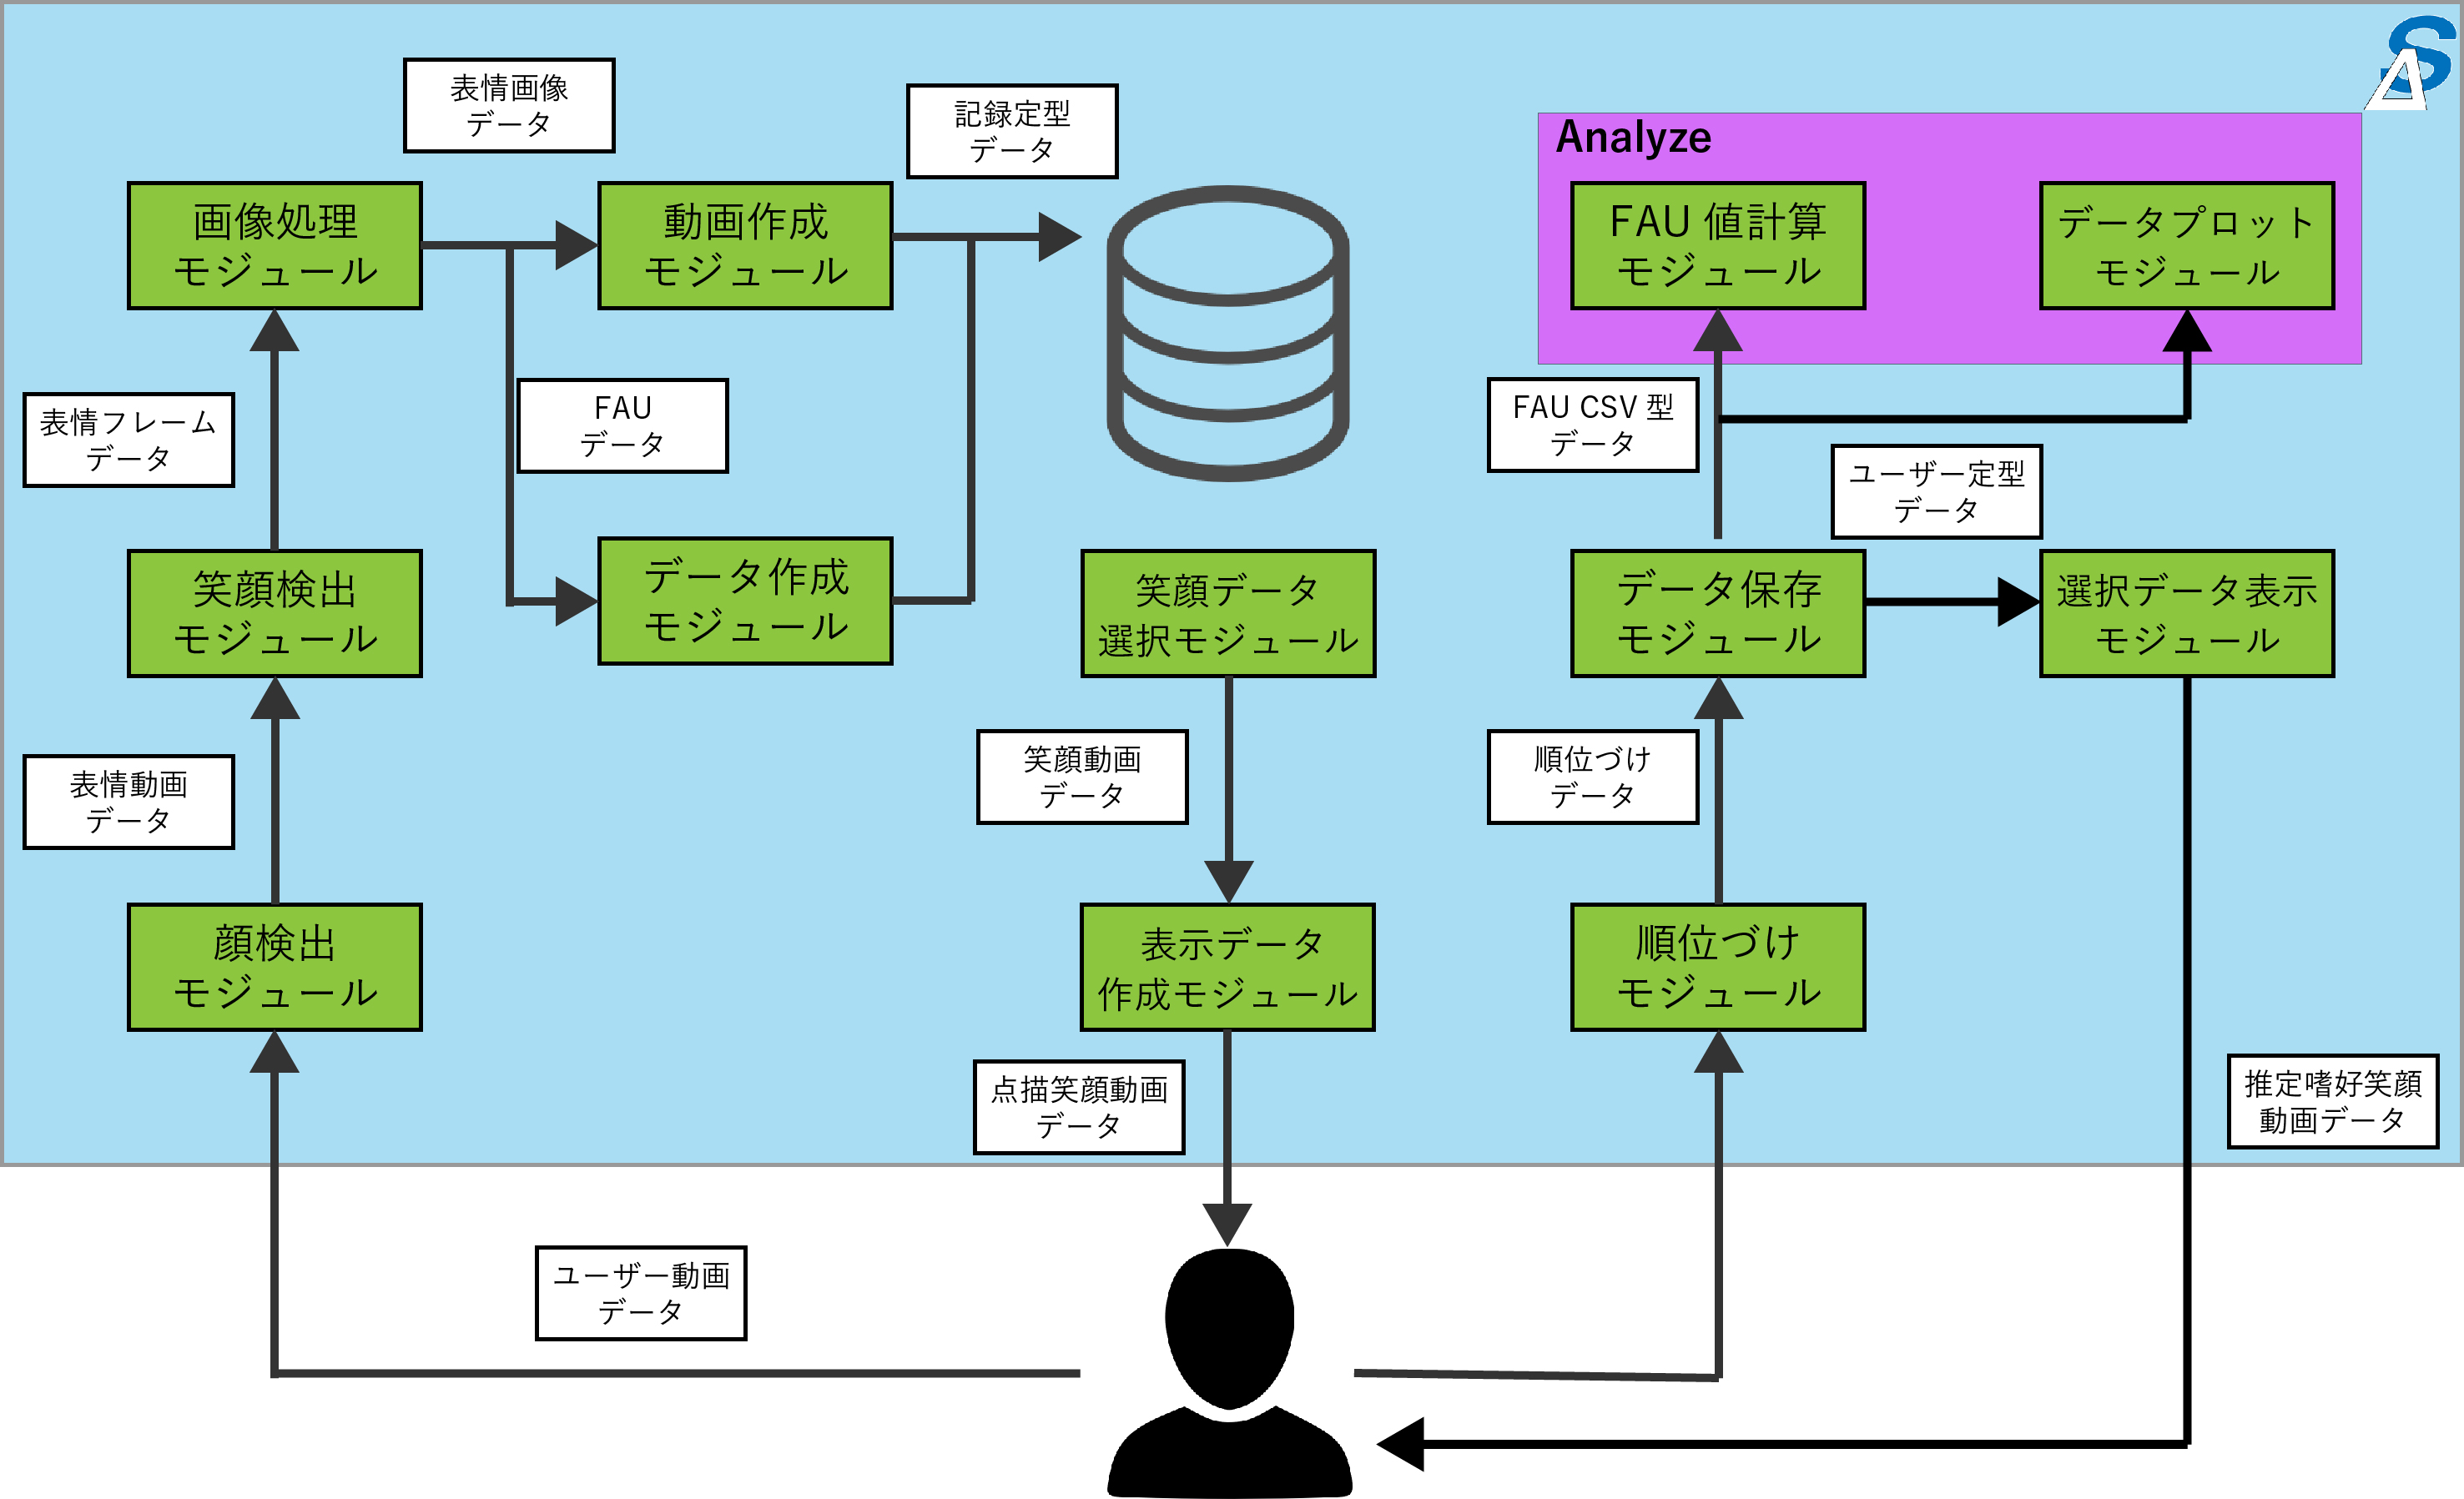
\includegraphics[width=150mm,bb=0 0 2953 1797]{system_architecture.jpg}}
    \end{center}
    \caption{システム構成図}
    \label{fig:system_architecture}
\end{figure}

\section{データ収集機能}
この節では, ユーザーエンドおよびデータ収集に必要な各モジュールの役割について説明する.
マシンスペックはMac Book Air, Core i5, メモリ8GB, ストレージ256GB, OS Mojave, version 10.14.5を使用し,
webカメラはLogicool C920r,ディスプレイはeizo sx2761w を使用する.

\subsection{顔検出モジュール}
パソコンのカメラ, もしくはwebカメラを起動して得た映像に対して顔の検出を行う.
ユーザーの顔のみを検出, トラッキングを行い, 特定領域のみに次の処理をかけることでシステムを軽量化する.
検出にはOpenCVのデフォルトのカスケードを使用し, Haar-like検出器を使って領域ごとに顔のパーツを検出し,
顔の領域を判別する.

\begin{figure}[htbp]
    \begin{center}
       \fbox{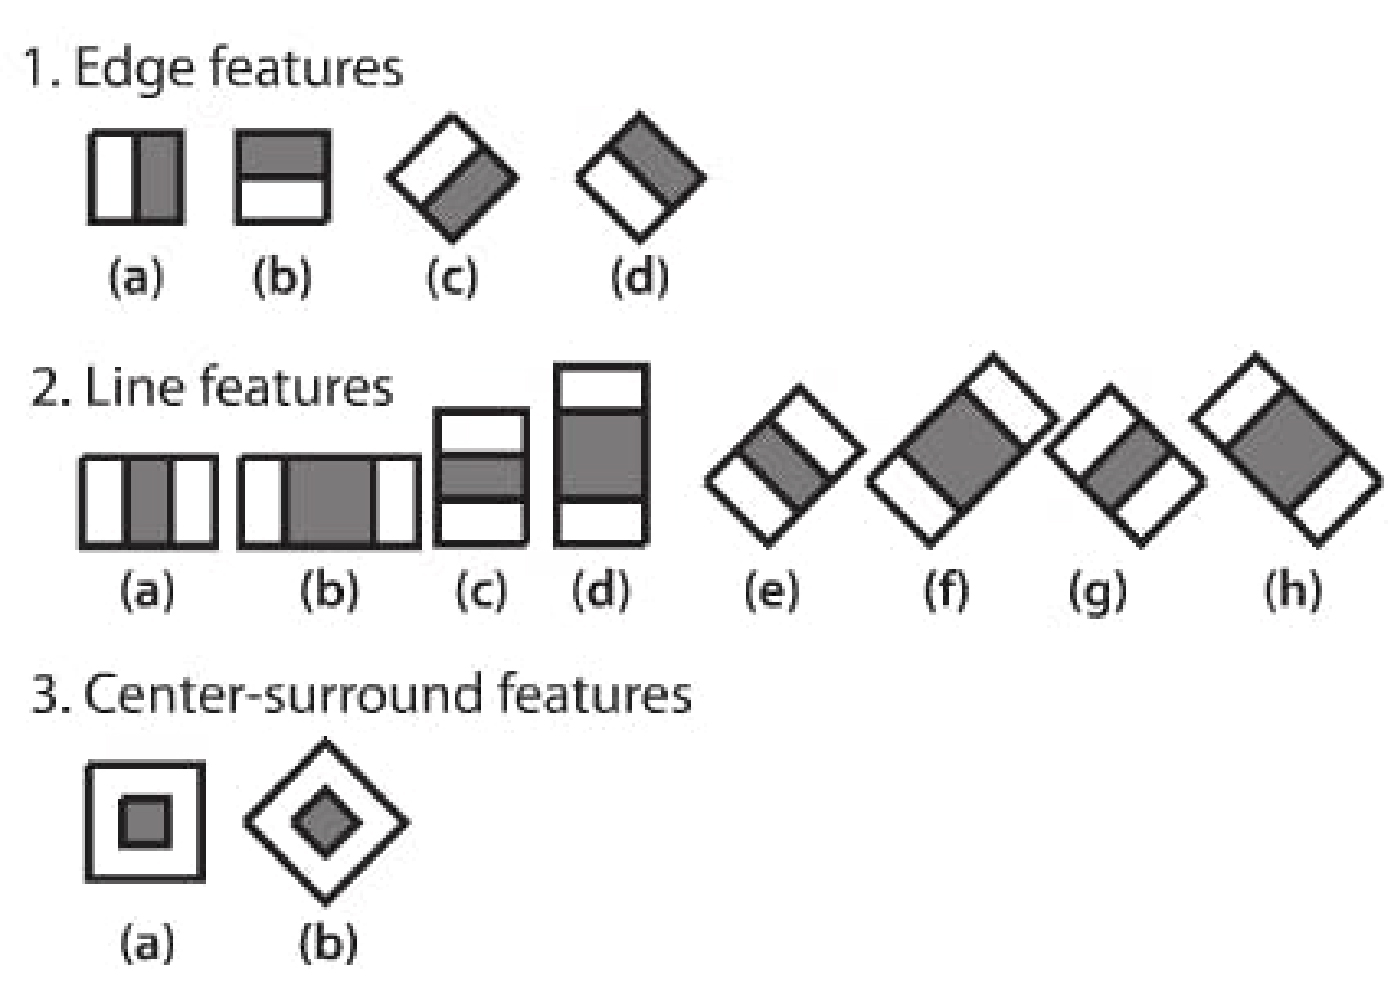
\includegraphics[width=150mm,bb=0 0 1395 989]{haarlikedetector.jpg}}
    \end{center}
    \caption{Harr\-like検出器}
    \label{fig:haarlikedetector}
\end{figure}

\subsection{笑顔検出モジュール}
顔検出モジュールで検出した顔の領域に対して, ユーザーの笑顔のタイミングを検出する処理を行う.
笑顔処理を動画全体にかけると誤検出や,  処理速度が落ちるため顔の領域のみに判別器をかける.
リアルタイム検出のために, 笑顔検出モジュールにはOpenCVのカスケードを使用する.
Haar-like検出器を使って口の領域に対して処理を行い, 口角の動きを検出し笑顔の判定を行う.
この検出方法の有効性については, 6章の予備実験において評価する.

\subsection{画像処理モジュール}
中立の表情から, 笑顔になるタイミングを連続時系列データでトータル20フレーム, そのうち笑顔は5フレーム保存し,
各フレームに対してOpenFaceのFacial Action Unit の処理を行う.
処理された結果は各フレームごとに, 705個のパラメータについての値をCSVファイルにて返される.
結果, 20個のCSVファイルが作成されるので, それらのファイルを統合し1つのファイルを作成し,
ユーザーの表情データとする.

\subsection{動画作成モジュール}
保存したフレームをつなぎ合わせて1秒の動画を作成する.
20fpsで検出し, 笑顔を連続5フレーム検出した動画を本システムの笑顔動画のフォーマットとする.
このフォーマットが表情遷移を記録する上で有効であるかどうかは6章の予備実験にて評価する.

\subsection{データ作成モジュール}
動画作成と同時に, 画像処理モジュールで算出したFacial Action UnitをCSVフォーマットで保存する.
笑顔動画およびCSVデータをユーザーごとにファイリングを行い, データベースへ笑顔動画とCSVデータを
紐づけて保存する.

\subsection{笑顔データ選択モジュール}
OpenFaceの開発者であるTadas \cite{tadas} によると,OpenFaceから取得可能なp\_scaleパラメータは,
顔のパーツのバランスを示している.
このパラメータは特徴点のx, y, zの3点座標を使用し, 判定モデルのベースとなっている平均顔との差分λであり,
この顔の形状と表情のアイデンティティーを示す値とされている.
以下の式, Xはモデル内における顔パーツの位置データの集まりを示している.

\begin{equation}
  X =
  \left[
  \begin{array}{cccccccccccc}
  X_1, & X_2, & ... & X_n, & Y_1, & Y_2, & ... & Y_n, & Z_1, & Z_2, & ... & Z_n \\
  \end{array}
  \right]
  ^{\mathrm{T}}
\end{equation}

\begin{figure}[htbp]
    \begin{center}
       \fbox{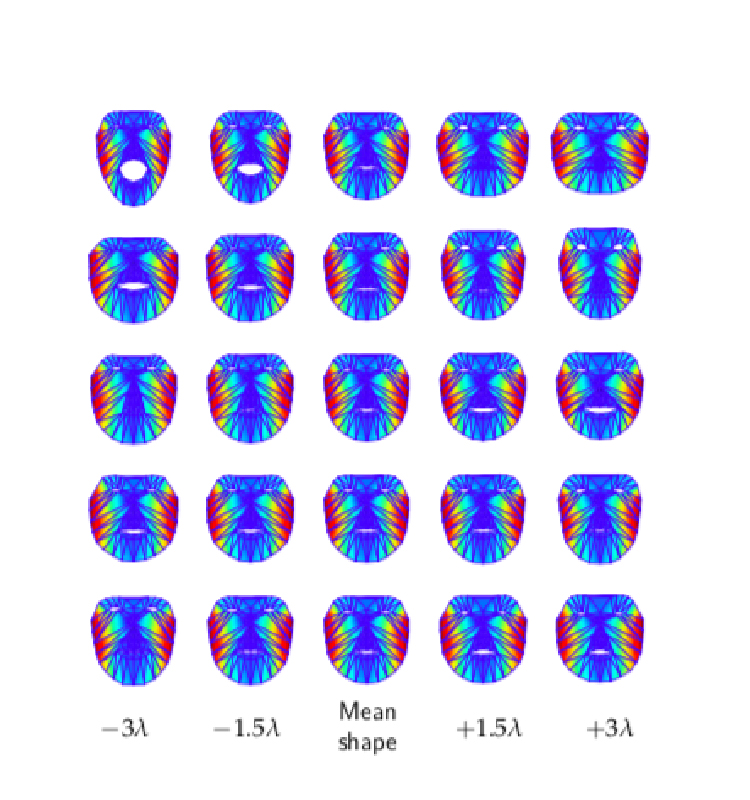
\includegraphics[width=150mm,bb=0 0 750 800]{face_balance.jpg}}
    \end{center}
    \caption{Multi\-PIEのデータセットから,λの値を顔に反映させたもの}
    \label{fig:face_balance}
\end{figure}

p\_scaleの値を算出し, 自分の笑顔動画データをふくむ5つのデータを選ぶ.
選択の基準は, ユーザーのp\_scaleとの差分を計算し,差分の最小値(ユーザー自身),第一四分位数,中央値,第三四分位数,最大値を選択する.

\subsection{表示データ作成モジュール}
表情の動き以外のバイアスを削減するために, 表情の動きは点描画のみで以下のようにな動画データを作成する.
顔の特徴点のみを抽出し, 表情の動きのみをユーザーに提示する.

\begin{figure}[htbp]
    \begin{center}
       \fbox{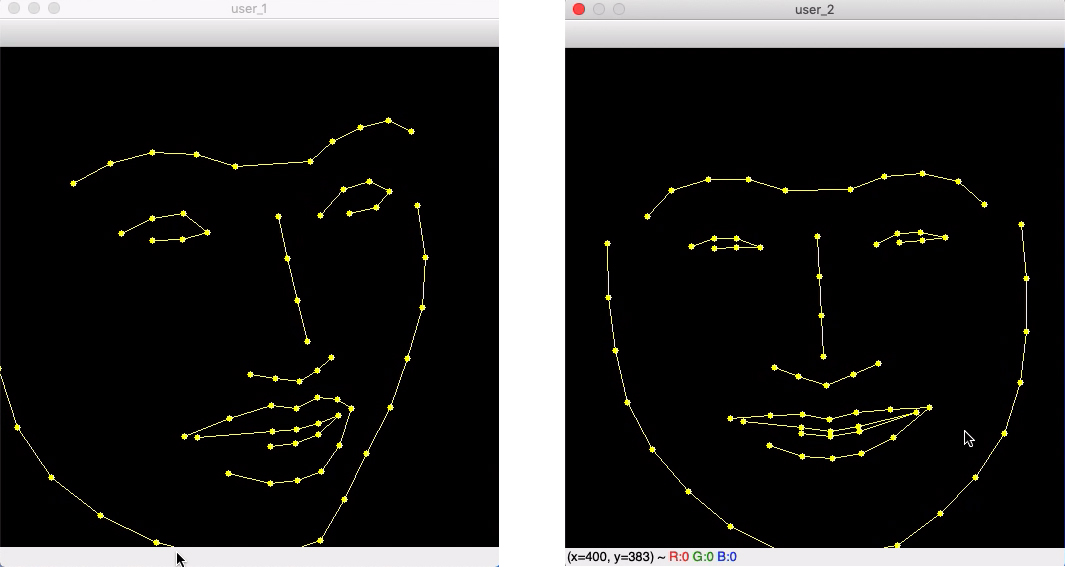
\includegraphics[width=150mm,bb=0 0 1065 567]{showdata.jpg}}
    \end{center}
    \caption{点描画笑顔動画データ}
    \label{fig:showdata}
\end{figure}

\subsection{順位づけモジュール}
ディスプレイに5種類の動画の中の2種類を表示し, 左右どちらの表情の動きが好みか選んでもらう.
左右比較を4回繰り返し, 各点描笑顔動画データに対して順位づけを行う.
選択した順位データと画像の保存先のpathを関連づけて保存することで,
のちのデータ整理をする際にユーザーごとのデータとしてファイリングを容易にすることができる.

\subsection{データ保存モジュール}
ユーザーの笑顔動画データ, FAU算出CVSデータ,5つの笑顔動画データへの順位づけデータ,ユーザーの
順位づけが一番高かった笑顔動画データおよびそのFAU算出CSVデータ,そして,ユーザーが順位づけした
その他の笑顔動画とそのFAU算出CSVデータを1つのディレクトリに格納し保存する.

\subsection{選択データ表示モジュール}
ユーザーの笑顔動画データと, 順位づけが一番高かった笑顔動画データを横にならべ動画データとし,
ユーザーに表示する. 本研究においては, 自身の笑顔と, 表情ベースにおける相手への嗜好分析を行う段階であるため,
実際にユーザーへフィードバックするデータは一番順位づけの高かった笑顔動画データのみとし,
その他の本システムで収集したユーザーのプライバシーが含まれる年齢などは公開しない.
将来的に, 本研究の結果を分析し, サービスや実証実験の場にて使用する時にはプライバシーポリシーに乗っ取りつつ,
情報開示を行った分析も行っていくこととする.


\section{データ分析機能}
本節では, 収集したデータを分析するためのモジュールについて説明をする.
データを収集したのち, 主にCSVファイルを使用して値を算出するための機能である.

%途中
\subsection{FAU値計算モジュール}
取得したcsvデータから分析に必要なデータを取り出し, 別の計算用のcsvファイルを作成する.
嗜好傾向分析に使用する笑顔のFAUの値は, FAU06(眼窩部眼輪筋),07(眼瞼部眼輪筋),12(大頬骨筋),25(翼突筋+顎二腹筋)の4種類を扱う.
各FAUはAU\_r(0から5のまでのスケール)とAU\_c(0と1の2極地)の2種類の値を持っているため, 合計8種類の値を生データから抽出する.
ユーザー自身および選ばれた笑顔動画データのFAUデータを抽出し, 最大値, 最小値, 値の範囲, 平均値, 中央値, 分散, 標準偏差, 不偏分散の値を計算する.
8種類の値をそれぞれのFAUデータに対して求め, 嗜好傾向との関連を考察する.


\subsection{データプロットモジュール}
FAU計算モジュールで算出した各ユーザーのFAUデータおよび選ばれた笑顔動画データのFAUデータの値をx軸にフレーム,y軸にFAUの値をプロットする.
視覚的にFAUの値を処理し, データ分析をする方針を立てる. また上昇傾向, 下降傾向などデータ全体の動きを把握する.

\section{まとめ}
本章ではDelta Smile Facial Survey Analyzer の設計, 各モジュールの役割について説明した.
次章では実際に作成したシステムの動きや, 工夫について説明をする.
